% This presentation is based on a Beamer theme from Seth Brown, distributed
% under the following license:
%
% ----------------------------------------------------------------------------
% This program can be redistributed and/or modified under the terms
% of the GNU Public License, version 3.
%
% Seth Brown, Ph.D.
% sethbrown@drbunsen.org

\documentclass[t,aspectratio=169]{beamer}

%\usepackage{xcolor}

% White on black scheme
\definecolor{lightbg}{HTML}{808080}     % 50% gray
\definecolor{mediumbg}{HTML}{666666}    % 60% gray
\definecolor{darkbg}{HTML}{333333}      % 80% gray
\definecolor{background}{HTML}{1A1A1A}  % 90% gray
\definecolor{foreground}{HTML}{FFFFFF}  % white

\definecolor{active1}{HTML}{FFE499}     % pale orange
\definecolor{active2}{HTML}{FF99FF}     % pale pink
\definecolor{active3}{HTML}{00FFFF}     % cyan

%\usepackage{xcolor}

% "chalkboard" scheme
%
% def mix(ac,bc,f): return "#%02X%02X%02X" % tuple([int((a * float(f)) + (b * (1.0 - f))) for a,b in zip(ac, bc)])

\definecolor{lightbg}{HTML}{AEC2B4}     % 40% tint of chalkboard green
\definecolor{mediumbg}{HTML}{153E29}
\definecolor{darkbg}{HTML}{1A3422}      % 50% shade of chalkboard green
\definecolor{background}{HTML}{356845}  % Chalkboard green
\definecolor{foreground}{HTML}{FFFFFF}  % white

\definecolor{active1}{HTML}{FAD48B}     % Orange Chalk
\definecolor{active2}{HTML}{BCDF8A}     % Green Chalk
\definecolor{active3}{HTML}{94C0CC}     % Blue Chalk

\usepackage{xcolor}

% "chalkboard" scheme
%
% def mix(ac,bc,f): return "#%02X%02X%02X" % tuple([int((a * float(f)) + (b * (1.0 - f))) for a,b in zip(ac, bc)])

\definecolor{lightbg}{HTML}{AEC2B4}     % 40% tint of chalkboard green
\definecolor{mediumbg}{HTML}{153E29}
\definecolor{darkbg}{HTML}{356845}      % 50% shade of chalkboard green 1A3422
\definecolor{background}{HTML}{1A3422}  % Chalkboard green 356845
\definecolor{foreground}{HTML}{FFFFFF}  % white

\definecolor{active1}{HTML}{FAD48B}     % Orange Chalk
\definecolor{active2}{HTML}{BCDF8A}     % Green Chalk
\definecolor{active3}{HTML}{94C0CC}     % Blue Chalk

\mode<presentation>{\usetheme{codeplay}}

% title slide definition
\title{Creating an SPMD Vectorizer for OpenCL\textsuperscript{TM} with LLVM}
\subtitle{LLVM 2015 Tutorial}
\author{Pierre-André Saulais \\ <pierre-andre@codeplay.com>}
\institute{Codeplay Software \\ @codeplaysoft}

\date{October 29, 2015}

\newcommand{\varying}[1]{\codeempha{#1}}
\newcommand{\uniform}[1]{\codeemphb{#1}}

\newcommand{\pointfor}[1]{\hspace{1em}\textbf{\codeemphb{{\fontspec{Cambria Math} +}}}\hspace{0.5em}#1}
\newcommand{\pointunkn}[1]{\hspace{1em}\textbf{?}\hspace{0.5em}#1}
\newcommand{\pointagainst}[1]{\hspace{1em}\textbf{\codeempha{{\textendash}}}\hspace{0.5em}#1}

\newcommand{\llvmlogo}[1]{\raisebox{-1.3ex}{\includegraphics[scale=#1]{images/LLVM_Logo.pdf}}\hspace{-0.3em}}
\newcommand{\llvmlogovec}[1]{\llvmlogo{#1}, \llvmlogo{#1}, \llvmlogo{#1}, \llvmlogo{#1}, \llvmlogo{#1}, \llvmlogo{#1}, \llvmlogo{#1}, \llvmlogo{#1}\hspace{0.3em}}

%%%%%%%%%%%%%%%%%%%%%%%%%%%%%%%%%%%%%%%%%%%%%%%%%%%%%%%%%%%%%%%%%%%%%%%%%%%%%%%%

\begin{document}

%\setbeamertemplate{background}
%{\includegraphics[width=\paperwidth,height=\paperheight]{dark_background_title.png}}
\setbeamertemplate{footline}[default]

\begin{frame}
  \vspace{4ex}
  \titlepage
\end{frame}

%%%%%%%%%%%%%%%%%%%%%%%%%%%%%%%%%%%%%%%%%%%%%%%%%%%%%%%%%%%%%%%%%%%%%%%%%%%%%%%%

\setbeamertemplate{background}{}
\setbeamertemplate{footline}[codeplaytheme]

\section*{Introduction}

\begin{frame}{What this tutorial is about}

\begin{minipage}[t]{0.70\linewidth}

\begin{itemize}  
    \item Vectorizing
    \begin{itemize}
        \item Transform whole functions using LLVM
        \item "Horizontal" vectorization (not loop-based)
    \end{itemize}  
    \item SPMD (Single Program, Multiple Data) Kernels
    \begin{itemize}
        \item Data-parallel execution model
        \item Compute frameworks like OpenCL\textsuperscript{TM} and CUDA\textsuperscript{TM}
    \end{itemize}
    \item for CPUs, DSPs,
    \begin{itemize}
        \item Explicitly programmed SIMD unit(s)
        \item Can execute both scalar and vector instructions
    \end{itemize}
    \item An introduction
    \begin{itemize}
        \item Create a basic vectorizer
    \end{itemize}
\end{itemize}

\end{minipage}\hspace{1em}\begin{minipage}[t]{0.25\linewidth}
\vspace{-3.5ex}
\center{\includegraphics[scale=0.07]{images/LLVM_Logo.pdf}}
\vspace{-2.5ex}\center{\includegraphics[scale=0.25]{images/OpenCL_Logo.png}}
\center{\includegraphics[scale=0.155]{images/CUDA.png}}

\end{minipage}

\end{frame}

%%%%%%%%%%%%%%%%%%%%%%%%%%%%%%%%%%%%%%%%%%%%%%%%%%%%%%%%%%%%%%%%%%%%%%%%%%%%%%%%

\begin{frame}{Overview}
\tableofcontents
\end{frame}

%%%%%%%%%%%%%%%%%%%%%%%%%%%%%%%%%%%%%%%%%%%%%%%%%%%%%%%%%%%%%%%%%%%%%%%%%%%%%%%%

\talkpart{1}{Background}
%%%%%%%%%%%%%%%%%%%%%%%%%%%%%%%%%%%%%%%%%%%%%%%%%%%%%%%%%%%%%%%%%%%%%%%%%%%%%%%%

\talksection{SPMD Execution Model}

\begin{frame}{SPMD Execution Model}

\begin{itemize}
    \item Data-parallel
    \begin{itemize}
        \item Work needs to be divided
    \end{itemize}
    
    \item Single program, scalar with implicit SIMD execution
    
    \item Multiple instances running in parallel
    \begin{itemize}
        \item Each instance working on different data
        \item On GPU, SIMD execution in lockstep
        \item On CPU, sequential execution within a core (naive approach)
    \end{itemize}
\end{itemize}

\begin{itemize}
    \item Simplistic example:
    \begin{itemize}
        \item Massive Online Course
        \item Compute the overall grade (GPA) of millions of students
        \item GPA is the weighted average of several grades
    \end{itemize}
\end{itemize}

\end{frame}

%% Kernel function has no return value, takes in buffers (arrays)
%% Vectorization does not change the signature for kernels
%% Can also vectorize "normal" functions, but this results in signature changes

%%%%%%%%%%%%%%%%%%%%%%%%%%%%%%%%%%%%%%%%%%%%%%%%%%%%%%%%%%%%%%%%%%%%%%%%%%%%%%%%

\begin{frame}{Division of Work}

\begin{itemize}
    \item Work-item:
    \begin{itemize}
        \item Unit of work
        \item One instance of a program
    \end{itemize}
    \item Work-items executed in parallel by Execution Units (threads)
    \item Dimensions
    \begin{itemize}
        \item 1D (array shape)
        \item 2D (grid shape)
        \item ...
    \end{itemize}
\end{itemize}

[graph]

\end{frame}

%%%%%%%%%%%%%%%%%%%%%%%%%%%%%%%%%%%%%%%%%%%%%%%%%%%%%%%%%%%%%%%%%%%%%%%%%%%%%%%%

\begin{frame}[fragile]{Single Program}

\begin{itemize}
    \item Kernel function
    \begin{itemize}
        \item Entry point for the computation
    \end{itemize}
    \item Executed once per work-item
    \begin{itemize}
        \item As if there was a loop around it
        \item Access to the iteration counter using \texttt{get\_global\_id(0)}
    \end{itemize}
\end{itemize}

\begin{codebox}
kernel void calc_gpa(global *float result, global *int grades, global *float weights,
                     int num_grades, int num_students) {
    int student_id = get_global_id(0);
    float gpa = 0.0;
    for (int i = 0; i < num_grades; i++) {
        int grade = grades[(i * num_students) + student_id];
        float weight = weights[i];
        gpa += (grade * weight);
    }
    result[student_id] = gpa;
}
\end{codebox}

\end{frame}

%%%%%%%%%%%%%%%%%%%%%%%%%%%%%%%%%%%%%%%%%%%%%%%%%%%%%%%%%%%%%%%%%%%%%%%%%%%%%%%%

\talksection{Vectorization}
\begin{frame}{Why Vectorize?}

\begin{itemize}
    \item Many executions units each executing one instance of a single program 
    \begin{itemize}
        \item Works well on GPU (many hardware EUs)
        \item Not so much on CPU (very few hardware EUs)
        \item CPU has to execute many work-items sequentially
    \end{itemize}
    \item Speed up this sequential computation using SIMD units
    \begin{itemize}
        \item Vertical Vectorization
        \item Horizontal Vectorization
    \end{itemize}
\end{itemize}

\end{frame}

%%%%%%%%%%%%%%%%%%%%%%%%%%%%%%%%%%%%%%%%%%%%%%%%%%%%%%%%%%%%%%%%%%%%%%%%%%%%%%%%

\begin{frame}{Vertical Vectorization}

\begin{itemize}
    \item Within a single work-item
    \begin{itemize}
        \item e.g. loops within a kernel
        \item In our example, the weighted average computation
        \end{itemize}
    \item Using the LLVM Loop Vectorizer
    \item However, not all kernels contain loops
\end{itemize}

[graph of work-items with vertical loops]

\end{frame}

%%%%%%%%%%%%%%%%%%%%%%%%%%%%%%%%%%%%%%%%%%%%%%%%%%%%%%%%%%%%%%%%%%%%%%%%%%%%%%%%

\begin{frame}{Horizontal Vectorization}

\begin{itemize}
    \item Across work-items
    \begin{itemize}
        \item Compute multiple work-items at the same time
        \item Take advantage of the execution model (single program, multiple data)
    \end{itemize}
\end{itemize}

[graph of work-items with horizontal arrows]

\end{frame}

%%%%%%%%%%%%%%%%%%%%%%%%%%%%%%%%%%%%%%%%%%%%%%%%%%%%%%%%%%%%%%%%%%%%%%%%%%%%%%%%

\begin{frame}{Vectorizer Comparison}

\begin{itemize}
    \item Loop Vectorizer
    \begin{itemize}
        \item Can be used for both vertical and horizontal vectorization
        \item Has to enforce dependencies between loop iterations
        \item Execution order is not specified, this is not needed
        \item Nested control-flow?
    \end{itemize}

    \item SLP Vectorizer
    \begin{itemize}
        \item Finds groups of similar scalar instructions (same opcode)
        \item Vertical vectorization
        \item Not all kernels contain this kind of code
    \end{itemize}

    \item SPMD Vectorizer
    \begin{itemize}
        \item Only supports horizontal vectorization
        \item Nested control-flow
        \item Not limited to a certain 'style' of code
    \end{itemize}
\end{itemize}

\end{frame}

%%%%%%%%%%%%%%%%%%%%%%%%%%%%%%%%%%%%%%%%%%%%%%%%%%%%%%%%%%%%%%%%%%%%%%%%%%%%%%%%

\begin{frame}{Glossary}

\begin{itemize}
    \item Work
    \begin{itemize}
        \item Work-item: unit of work to execute in parallel.
        \item Instance: State of one work-item.
        \item (SIMD) Lane: Execution of one instance, after vectorization.
        \end{itemize}
        
    \item Data
    \begin{itemize}
        \item Packet: Contains several values/instructions, one per SIMD lane. Corresponds to one value/instruction in the original kernel.
        \item \uniform{Uniform}: Packet where values are identical for all lanes.
        \item \varying{Varying}: Packet where values are not identical for all lanes.
        \end{itemize}

    \item Control Flow
    \begin{itemize}
        \item \uniform{Uniform}: Branch taken by all lanes.
        \item \varying{Divergent}: Branch taken by some lanes. Requires special handling (No SIMD branching)
    \end{itemize}
\end{itemize}

\end{frame}


\talkpart{2}{Implementing a SPMD Vectorizer}
%%%%%%%%%%%%%%%%%%%%%%%%%%%%%%%%%%%%%%%%%%%%%%%%%%%%%%%%%%%%%%%%%%%%%%%%%%%%%%%%

\talksection{Overview}

\begin{frame}{Structure}

\begin{itemize}
    \item Pipeline design
    \begin{itemize}
        \item $F$ is repeatedly transformed by different stages
        \item Stages are independent from each other
        \item Each stage consists of one or more IR passes
        \item Most stages require some analysis
    \end{itemize}
    \item Analyses
    \begin{itemize}
        \item Capture information about the IR to vectorize
        \item May need updating after a stage (stale information)
        \item May depend on other analyses
    \end{itemize}
\end{itemize}

\center{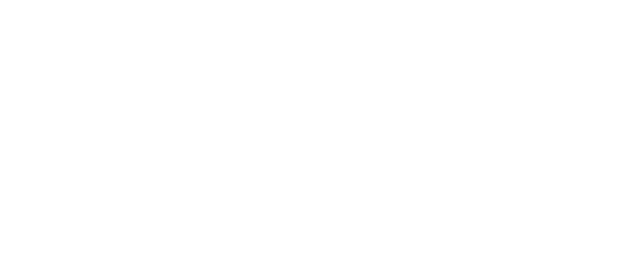
\includegraphics[width=0.8\textwidth]{images/stages.pdf}}

\end{frame}

%%%%%%%%%%%%%%%%%%%%%%%%%%%%%%%%%%%%%%%%%%%%%%%%%%%%%%%%%%%%%%%%%%%%%%%%%%%%%%%%

\begin{frame}{Analysis Examples}

\begin{itemize}
    \item Uniform Value Analysis
    \begin{itemize}
        \item Marks values as either \uniform{uniform} or \varying{varying}
    \end{itemize}

    \item Control Flow Analysis
    \begin{itemize}
        \item Determines which basic blocks are \varying{divergent}
        \item Builds a Control Dependency Graph
    \end{itemize}
    
    \item SIMD Width Analysis
    \begin{itemize}
        \item Chooses a 'good' width $N$ based on register/instruction usage
    \end{itemize}
    
    \item ...
\end{itemize}

\end{frame}

%%%%%%%%%%%%%%%%%%%%%%%%%%%%%%%%%%%%%%%%%%%%%%%%%%%%%%%%%%%%%%%%%%%%%%%%%%%%%%%%

\begin{frame}{Implementation Level: IR or MI?}

\begin{itemize}
    \item IR Level
    \begin{itemize}
        \item \pointfor{Use-def graph and \texttt{RAUW} make for straightforward transformations}
        \item \pointfor{Easy to target multiple platforms}
        \item \pointunkn{Generally higher-level (simpler implementation?)}
        \item \pointagainst{Platform-specific features more difficult to use}
        \item \pointagainst{Predication only for select operations (select, load/stores)}
    \end{itemize}

    \item MachineInstr level
    \begin{itemize}
        \item \pointfor{Easy to use platform-specific features (e.g. predication, mask registers)}
        \item \pointunkn{Generally lower-level (more powerful?)}
        \item \pointagainst{More platform-specific code}
        \item \pointagainst{Graph-based transformations not as straightforward}
    \end{itemize}
    
\end{itemize}

\end{frame}

%%%%%%%%%%%%%%%%%%%%%%%%%%%%%%%%%%%%%%%%%%%%%%%%%%%%%%%%%%%%%%%%%%%%%%%%%%%%%%%%

%\begin{frame}{Implementation strategy}
%
%% TODO: Skip slide?
%\begin{itemize}
%    \item Create test kernels
%    \begin{itemize}
%        \item Start with very simple kernels (e.g. copy buffer, add two buffers)
%        \item Gradually add more features (e.g. non-sequential memory accesses, vector instructions, etc)
%    \end{itemize}
%
%    
%    \item Suggested implementation order
%    \begin{itemize}
%        \item Preparation and packetization first (required for simplest kernels)
%        \item Then easier features: builtins, memory addressing, scalarization, instantiation
%        \item More complex features last: control flow, optimizations
%    \end{itemize}
%\end{itemize}
%
%\end{frame}

\talksection{Packetization Stage}

\begin{frame}{Packetization Overview}

\begin{itemize}
    \item Stage that does the actual vectorization: $<F, N> \rightarrow VF_N$
    \begin{itemize}
        \item Needs a vectorization factor $N$ (SIMD width)
        \item Calling $VF_N$ is like calling $F$, but $N$ times
        \item Straightforward thanks to preparation from previous stages
    \end{itemize}
    
    \item This is done per-instruction, for the whole function
    \begin{itemize}
        \item Instructions that define a value: define $N$ values, one for each instance
        \item Instructions with side effects: perform side effects for each instance
        \item New instruction has the same opcode but different types
    \end{itemize}
    
    \item Only \varying{varying} instructions need packetization
    \begin{itemize}
        \item \uniform{Uniform} instructions can remain scalar, executed once per work-group
        \item Requires \emph{Uniform Value Analysis} to know which instructions to vectorize
    \end{itemize}
    
\end{itemize}

\end{frame}

%%%%%%%%%%%%%%%%%%%%%%%%%%%%%%%%%%%%%%%%%%%%%%%%%%%%%%%%%%%%%%%%%%%%%%%%%%%%%%%%

\begin{frame}{Uniform Value Analysis}

\begin{itemize}
    \item Finds 'root' values
    \begin{itemize}
        \item \varying{Varying} values with no \varying{varying} operand
        \item Example: \varying{get\_global\_id(0)} has a different value for each isntance
    \end{itemize}
    \item Marks each IR value as \uniform{uniform} or \varying{varying}
    \begin{itemize}
        \item All values start as \uniform{uniform}
        \item Marking a value as \varying{varying} causes all users to also be marked \varying{varying}
        \item Marking is done recursively, starting with roots
        \item Values are marked before their users, to avoid cycles (phi nodes)
    \end{itemize}
\end{itemize}

\end{frame}

%%%%%%%%%%%%%%%%%%%%%%%%%%%%%%%%%%%%%%%%%%%%%%%%%%%%%%%%%%%%%%%%%%%%%%%%%%%%%%%%

\begin{frame}[fragile]{Uniform Value Analysis}

Example that combines \uniform{uniform} and \varying{varying} values:

\begin{codebox}[commandchars=\\\[\]]
kernel void add_uniform(global int *\uniform[dst], global int *\uniform[src], int \uniform[alpha]) {
    int \varying[tid] = \varying[get_global_id](0);
    \uniform[dst]\idx[\varying[tid]] = \uniform[src]\idx[\varying[tid]] + (\uniform[alpha] - \uniform[1]);
}
\end{codebox}

\begin{codebox}[commandchars=\\\[\]]
define void @add_uniform(i32* \uniform[%dst], i32* \uniform[%src], i32 \uniform[%alpha]) {
entry:
  \varying[%tid] = i32 \varying[@get_global_id(i32 0)]
  \varying[%arrayidx] = getelementptr i32* \uniform[%src], i32 \varying[%tid]
  \varying[%tmp] = load i32* \varying[%arrayidx], align 4
  \uniform[%sub] = sub i32 \uniform[%alpha], \uniform[1]
  \varying[%add] = add i32 \uniform[%sub], \varying[%tmp]
  \varying[%arrayidx2] = getelementptr i32* \uniform[%dst], i32 \varying[%tid]
  store i32 \varying[%add1], i32* \varying[%arrayidx2], align 4
  ret void
}
\end{codebox}

\end{frame}

%%%%%%%%%%%%%%%%%%%%%%%%%%%%%%%%%%%%%%%%%%%%%%%%%%%%%%%%%%%%%%%%%%%%%%%%%%%%%%%%

\begin{frame}[c]{UVA Example: Start}

\center{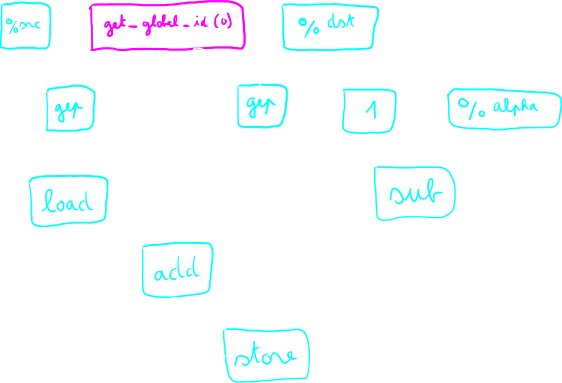
\includegraphics[scale=0.6]{images/uva-example-start.pdf}}

\end{frame}

%%%%%%%%%%%%%%%%%%%%%%%%%%%%%%%%%%%%%%%%%%%%%%%%%%%%%%%%%%%%%%%%%%%%%%%%%%%%%%%%

\begin{frame}[c]{UVA Example: Propagation}

\center{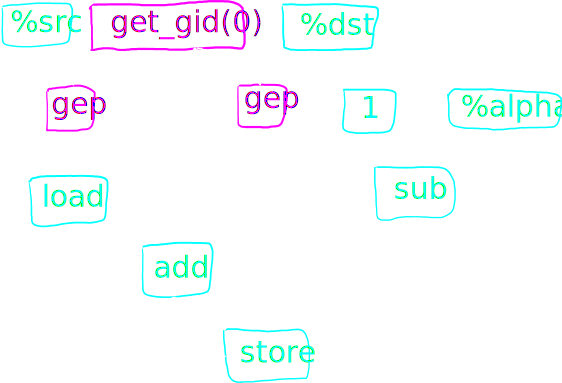
\includegraphics[scale=0.6]{images/uva-example-interm.pdf}}

\end{frame}

%%%%%%%%%%%%%%%%%%%%%%%%%%%%%%%%%%%%%%%%%%%%%%%%%%%%%%%%%%%%%%%%%%%%%%%%%%%%%%%%

\begin{frame}[c]{UVA Example: End}

\center{\includegraphics[scale=0.6]{images/uva-example-end.pdf}}

\end{frame}

%%%%%%%%%%%%%%%%%%%%%%%%%%%%%%%%%%%%%%%%%%%%%%%%%%%%%%%%%%%%%%%%%%%%%%%%%%%%%%%%

\begin{frame}{Memory Addressing}

\begin{itemize}
    %\item \varying{get\_global\_id(0)} was not packetized to a sequence of IDs. Why?
    \item Loads and stores are packetized according to the addressing mode
    \begin{itemize}
        \item Each operation can access $N$ memory elements
        \item Address usually has the form `\uniform{base} + \varying{offset}'
        \item Need to evaluate the offset for each of the $N$ lanes
    \end{itemize}
    
    \item How are these elements laid out in memory?
    \begin{itemize}
        \item The layout affects how operations are packetized
        \item Most common layouts can be described with a single \emph{stride}
    \end{itemize}
    
    \item Stride is the distance between successive elements
    \begin{itemize}
        \item Expressed in number of elements
        \item "How many elements are skipped in memory to get to the next one"
        \item One means elements are consecutive
        \item Negative means memory offsets are decreasing
    \end{itemize}
    
    %\item Not all kinds of memory operations can be expressed in IR
    %\begin{itemize}
    %    \item Generate calls to internal builtins
    %    \item Internal builtins can be implemented for each target as supported 
    %\end{itemize}
    
\end{itemize}

\end{frame}

%%%%%%%%%%%%%%%%%%%%%%%%%%%%%%%%%%%%%%%%%%%%%%%%%%%%%%%%%%%%%%%%%%%%%%%%%%%%%%%%

\begin{frame}[fragile]{Uniform Memory Addressing}

%% TODO: Use 1 as offset, update the diagram
\begin{itemize}
    \item Constant $Stride = 0$
    \item Packetized offset is \uniform{uniform} (e.g. $<0, 0, 0, 0>$)
    \item Transformed to a regular \emph{scalar} load or store
\end{itemize}

\begin{minipage}[t]{0.40\linewidth}
    \vspace{0.1ex}
    \begin{codebox}[commandchars=\\\[\]]

global int \uniform[*src];
int \uniform[x] = \uniform[src]\idx[\uniform[0]];






    \end{codebox}
\end{minipage}
\begin{minipage}[t]{0.49\linewidth}
    \begin{figure}
        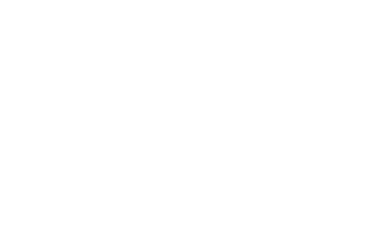
\includegraphics[scale=0.5]{images/uniform-access.pdf}
    \end{figure}
\end{minipage}

\end{frame}

%%%%%%%%%%%%%%%%%%%%%%%%%%%%%%%%%%%%%%%%%%%%%%%%%%%%%%%%%%%%%%%%%%%%%%%%%%%%%%%%

\begin{frame}[fragile]{Sequential Memory Addressing}

\begin{itemize}
    \item Constant $Stride = 1$
    \item Packetized offset is a sequence like $<0, 1, 2, 3>$
    \item Transformed to a regular \emph{vector} load or store
\end{itemize}

\begin{minipage}[t]{0.40\linewidth}
    \vspace{0.1ex}
    \begin{codebox}[commandchars=\\\[\]]

global int \uniform[*src];
int \varying[tid] = \varying[get_global_id(0)];
int \varying[x] = \uniform[src]\idx[\varying[tid]];





    \end{codebox}
\end{minipage}
\hspace{1em}
\begin{minipage}[t]{0.49\linewidth}
    \begin{figure}
        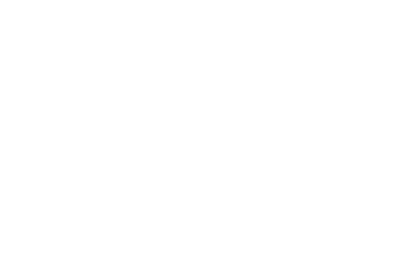
\includegraphics[scale=0.5]{images/sequential-access.pdf}
    \end{figure}
\end{minipage}

\end{frame}

%%%%%%%%%%%%%%%%%%%%%%%%%%%%%%%%%%%%%%%%%%%%%%%%%%%%%%%%%%%%%%%%%%%%%%%%%%%%%%%%

\begin{frame}[fragile]{Interleaved Memory Addressing}

\begin{itemize}
    \item Constant $Stride > 1$
    \item Packetized offset is a sequence like $<0, 2, 4, 6>$
    \item Transformed to an \emph{interleaved} load or store
\end{itemize}

\begin{minipage}[t]{0.40\linewidth}
    \vspace{0.1ex}
    \begin{codebox}[commandchars=\\\[\]]
    
global int \uniform[*src];
int \varying[tid] = \varying[get_global_id(0)];
int \varying[even] = \uniform[src]\idx[\varying[tid] * \uniform[2]];
int \varying[odd] = \uniform[src]\idx[(\varying[tid] * \uniform[2]) + \uniform[1]];




    \end{codebox}
\end{minipage}
\hspace{1em}
\begin{minipage}[t]{0.49\linewidth}
    \begin{figure}
        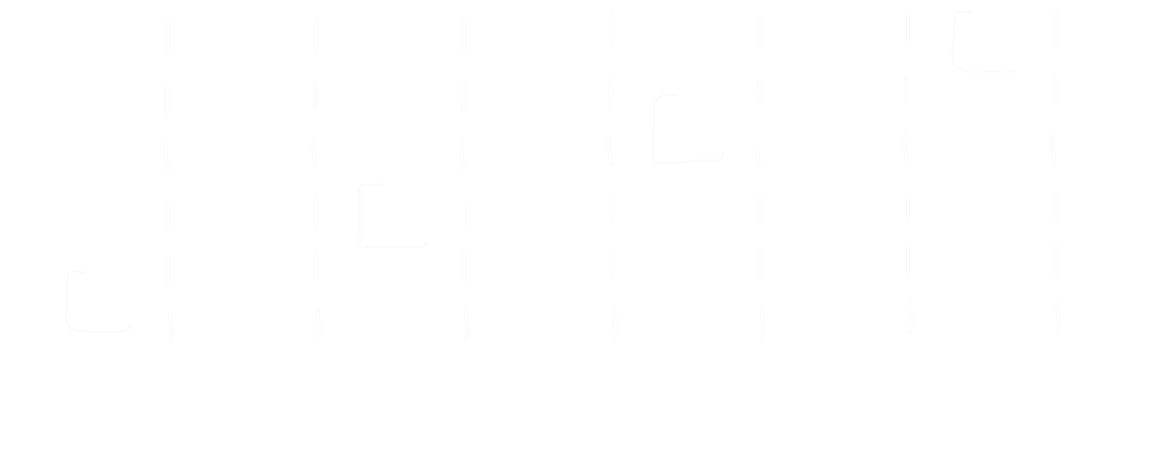
\includegraphics[scale=0.5]{images/interleaved-access.pdf}
    \end{figure}
\end{minipage}

\end{frame}

%%%%%%%%%%%%%%%%%%%%%%%%%%%%%%%%%%%%%%%%%%%%%%%%%%%%%%%%%%%%%%%%%%%%%%%%%%%%%%%%

\begin{frame}[fragile]{Arbitrary Memory Addressing}

\begin{itemize}
    \item Variable stride
    \item Packetized offset can be any sequence (e.g. $<0, 3, 7, 3>$)
    \item Transformed to a \emph{gather} load or \emph{scatter} store
\end{itemize}

\begin{minipage}[t]{0.40\linewidth}
    \vspace{0.1ex}
    \begin{codebox}[commandchars=\\\[\]]
    
global int \uniform[*src];
global int \uniform[*map];
int \varying[tid] = \varying[get_global_id(0)];
int \varying[x] = \uniform[src]\idx[\uniform[map]\idx[\varying[tid]]];




    \end{codebox}
\end{minipage}
\hspace{1em}
\begin{minipage}[t]{0.49\linewidth}
    \begin{figure}
        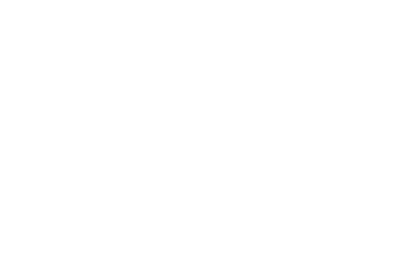
\includegraphics[scale=0.5]{images/arbitrary-access.pdf}
    \end{figure}
\end{minipage}

\end{frame}

%%%%%%%%%%%%%%%%%%%%%%%%%%%%%%%%%%%%%%%%%%%%%%%%%%%%%%%%%%%%%%%%%%%%%%%%%%%%%%%%

\begin{frame}{Packetization Process}

\begin{itemize}
    \item Find leaves
    \begin{itemize}
        \item Leaves allow \varying{varying} values to 'escape' from the function, they are:
        \item Store instructions (\varying{varying} operand)
        \item Call instructions (\varying{varying} operand, or call has no use)
        \item Return instructions
    \end{itemize}
\end{itemize}

\begin{itemize}
    \item Recursively packetize leaves and their operands
    \begin{itemize}
        \item Broadcast \uniform{uniform} values (e.g. argument, constants)
        \item Replace \varying{get\_global\_id(0)} with a vector of IDs
        \item Packetize operands first, then instruction (top-down)
        \item Cache packetized values to prevent duplication
    \end{itemize}
\end{itemize}

\begin{itemize}
    \item Delete original scalar instructions if dead
\end{itemize}

\end{frame}

%%%%%%%%%%%%%%%%%%%%%%%%%%%%%%%%%%%%%%%%%%%%%%%%%%%%%%%%%%%%%%%%%%%%%%%%%%%%%%%%

\begin{frame}[c]{Packetization Example}

\center{\includegraphics[scale=0.55]{images/uva-example-end.pdf}}

\end{frame}

%%%%%%%%%%%%%%%%%%%%%%%%%%%%%%%%%%%%%%%%%%%%%%%%%%%%%%%%%%%%%%%%%%%%%%%%%%%%%%%%

\begin{frame}[c]{Packetization Example}

\center{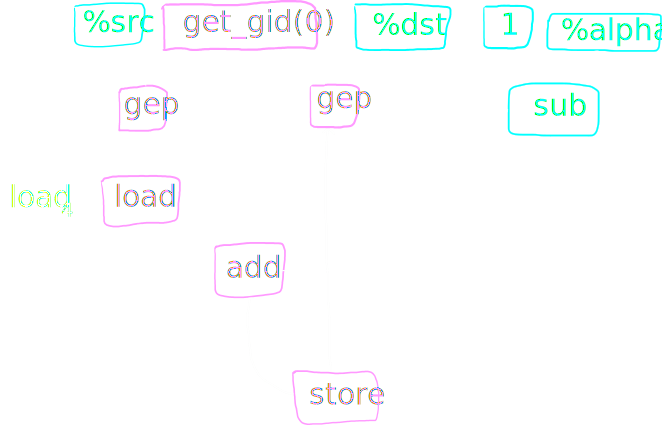
\includegraphics[scale=0.55]{images/packetization-1.pdf}}

\end{frame}

%%%%%%%%%%%%%%%%%%%%%%%%%%%%%%%%%%%%%%%%%%%%%%%%%%%%%%%%%%%%%%%%%%%%%%%%%%%%%%%%

\begin{frame}[c]{Packetization Example}

\center{\includegraphics[scale=0.55]{images/packetization-2.pdf}}

\end{frame}

%%%%%%%%%%%%%%%%%%%%%%%%%%%%%%%%%%%%%%%%%%%%%%%%%%%%%%%%%%%%%%%%%%%%%%%%%%%%%%%%

\begin{frame}[c]{Packetization Example}

\center{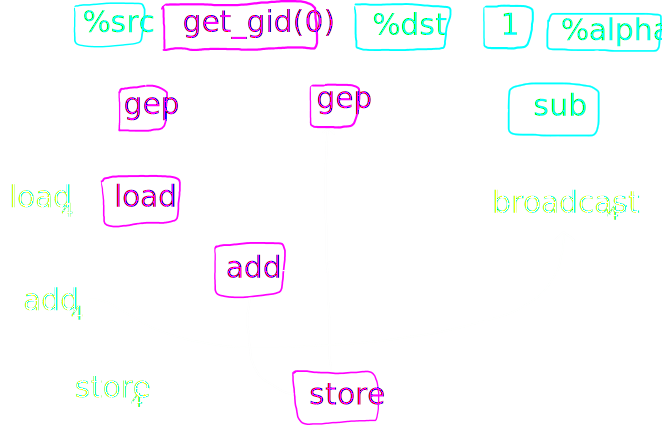
\includegraphics[scale=0.55]{images/packetization-3.pdf}}

\end{frame}

%%%%%%%%%%%%%%%%%%%%%%%%%%%%%%%%%%%%%%%%%%%%%%%%%%%%%%%%%%%%%%%%%%%%%%%%%%%%%%%%

\begin{frame}[c]{Packetization Example}

\center{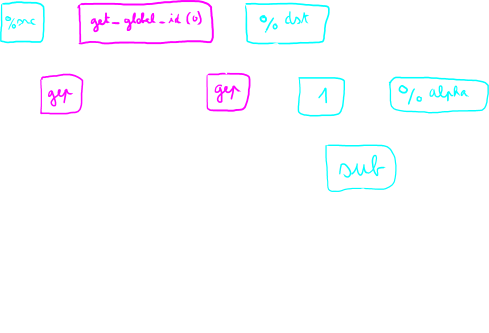
\includegraphics[scale=0.6]{images/packetization-4.pdf}}

\end{frame}

%%%%%%%%%%%%%%%%%%%%%%%%%%%%%%%%%%%%%%%%%%%%%%%%%%%%%%%%%%%%%%%%%%%%%%%%%%%%%%%%

\begin{frame}[fragile]{Packetization Example}

\begin{codebox}[commandchars=\\\[\]]
define void @__v4_add_uniform(i32* \uniform[%dst], i32* \uniform[%src], i32 \uniform[%alpha]) {
entry:
  \varying[%tid] = call i32 \varying[@get_global_id(i32 0)]
  \varying[%arrayidx] = getelementptr i32* \uniform[%src], i32 \varying[%tid]
  \varying[%0] = bitcast i32* \varying[%arrayidx] to <4 x i32>*
  \varying[%1] = load <4 x i32>* \varying[%0], align 4

  ; Broadcast (alpha - 1) to a vector
  \uniform[%sub] = sub i32 \uniform[%alpha], \uniform[1]
  \uniform[%insert] = insertelement <4 x i32> undef, i32 \uniform[%sub], i32 0
  \uniform[%broadcast_sub] = shufflevector <4 x i32> \uniform[%insert], ...

  \varying[%add] = add nsw <4 x i32> \uniform[%broadcast_sub], \varying[%1]

  \varying[%arrayidx2] = getelementptr i32* \uniform[%dst], i32 \varying[%tid]
  \varying[%2] = bitcast i32* \varying[%arrayidx2] to <4 x i32>*
  store <4 x i32> \varying[%add], <4 x i32>* \varying[%2], align 4
  ret void
}
\end{codebox}

\end{frame}

%%%%%%%%%%%%%%%%%%%%%%%%%%%%%%%%%%%%%%%%%%%%%%%%%%%%%%%%%%%%%%%%%%%%%%%%%%%%%%%%

\begin{frame}[fragile]{Packetizing Phi nodes}

\begin{itemize}
    \item Phi nodes can introduce cycles in the use/def graph
    \begin{itemize}
        \item Phi operands that reference the same phi
        \item Example: reduction variables
    \end{itemize}
    \item Break the cycle by creating 'empty' phi nodes
    \item Packetize operands of phi nodes after leaves have been packetized
\end{itemize}

\vspace{2ex}
\hspace{1em}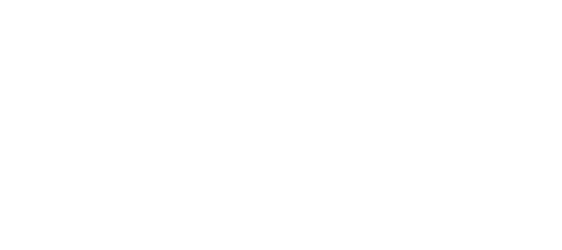
\includegraphics[scale=0.5]{images/phi-packetization.pdf}

\end{frame}

\talksection{Scalarization Stage}

\begin{frame}{Scalarization Overview}

\begin{itemize}
    \item What does it do?
    \item Requires scalarization analysis
\end{itemize}

\end{frame}

%%%%%%%%%%%%%%%%%%%%%%%%%%%%%%%%%%%%%%%%%%%%%%%%%%%%%%%%%%%%%%%%%%%%%%%%%%%%%%%%

\begin{frame}{Scalarization Analysis}

\begin{itemize}
    \item Looks for vector instructions
    \begin{itemize}
        \item Leaves that define vector values, vector stores
        \item Vector extractions
        \item Vector -> scalar bitcasts
    \end{itemize}
    
\end{itemize}

\end{frame}

%%%%%%%%%%%%%%%%%%%%%%%%%%%%%%%%%%%%%%%%%%%%%%%%%%%%%%%%%%%%%%%%%%%%%%%%%%%%%%%%

\begin{frame}{Scalarization Process}


\end{frame}

%%%%%%%%%%%%%%%%%%%%%%%%%%%%%%%%%%%%%%%%%%%%%%%%%%%%%%%%%%%%%%%%%%%%%%%%%%%%%%%%

\begin{frame}{Scalarization Example}


\end{frame}

\talksection{Control Flow Conversion Stage}

\begin{frame}{Control Flow Conversion Overview}

\begin{itemize}
    \item What does it do?
    \item Why is it needed?
\end{itemize}

\end{frame}

%%%%%%%%%%%%%%%%%%%%%%%%%%%%%%%%%%%%%%%%%%%%%%%%%%%%%%%%%%%%%%%%%%%%%%%%%%%%%%%%

\begin{frame}{Control Flow Conversion: if}

\end{frame}

%%%%%%%%%%%%%%%%%%%%%%%%%%%%%%%%%%%%%%%%%%%%%%%%%%%%%%%%%%%%%%%%%%%%%%%%%%%%%%%%

\begin{frame}{Mask Generation}

\end{frame}

%%%%%%%%%%%%%%%%%%%%%%%%%%%%%%%%%%%%%%%%%%%%%%%%%%%%%%%%%%%%%%%%%%%%%%%%%%%%%%%%

\begin{frame}{Applying Masks}

\end{frame}

%%%%%%%%%%%%%%%%%%%%%%%%%%%%%%%%%%%%%%%%%%%%%%%%%%%%%%%%%%%%%%%%%%%%%%%%%%%%%%%%

\begin{frame}{Masked Memory Operations}

\end{frame}

%%%%%%%%%%%%%%%%%%%%%%%%%%%%%%%%%%%%%%%%%%%%%%%%%%%%%%%%%%%%%%%%%%%%%%%%%%%%%%%%

\begin{frame}{Phi Conversion}

\end{frame}

%%%%%%%%%%%%%%%%%%%%%%%%%%%%%%%%%%%%%%%%%%%%%%%%%%%%%%%%%%%%%%%%%%%%%%%%%%%%%%%%

\begin{frame}{CFG Linearization}

\end{frame}

%%%%%%%%%%%%%%%%%%%%%%%%%%%%%%%%%%%%%%%%%%%%%%%%%%%%%%%%%%%%%%%%%%%%%%%%%%%%%%%%

\begin{frame}{Control Flow Conversion: loops}

\end{frame}

%%%%%%%%%%%%%%%%%%%%%%%%%%%%%%%%%%%%%%%%%%%%%%%%%%%%%%%%%%%%%%%%%%%%%%%%%%%%%%%%

\begin{frame}{Finding Loop Live Variables}

\end{frame}

%%%%%%%%%%%%%%%%%%%%%%%%%%%%%%%%%%%%%%%%%%%%%%%%%%%%%%%%%%%%%%%%%%%%%%%%%%%%%%%%

\begin{frame}{Merging Loop Live Variables}

\end{frame}


%\talkpart{3}{Going further}
%%%%%%%%%%%%%%%%%%%%%%%%%%%%%%%%%%%%%%%%%%%%%%%%%%%%%%%%%%%%%%%%%%%%%%%%%%%%%%%%%

\begin{frame}{SIMD Width Detection}

\end{frame}

%%%%%%%%%%%%%%%%%%%%%%%%%%%%%%%%%%%%%%%%%%%%%%%%%%%%%%%%%%%%%%%%%%%%%%%%%%%%%%%%

\begin{frame}{Vectorizing Builtin Function Calls}

% Builtin: the vectorizer has some knowledge of scalar -> vector function mapping

\end{frame}

%%%%%%%%%%%%%%%%%%%%%%%%%%%%%%%%%%%%%%%%%%%%%%%%%%%%%%%%%%%%%%%%%%%%%%%%%%%%%%%%

\begin{frame}{Vectorizing Builtin Functions}

% By vectorizing the builtin's body
% This changes the function signature (return value, some arguments)
% Builtin: the vectorizer has some knowledge of which arguments need packetization
% Need argument placeholders (cloning required)
% Packetized arguments are roots (Uniform Value Analysis)
% Return instructions are leaves (Packetization Stage)

\end{frame}

%%%%%%%%%%%%%%%%%%%%%%%%%%%%%%%%%%%%%%%%%%%%%%%%%%%%%%%%%%%%%%%%%%%%%%%%%%%%%%%%

\begin{frame}{Vectorizing User Functions (No Side-Effects)}

% Similar to builtin functions, but with no knowledge of whether arguments need
% packetization. Need to analyze this for each call site.

\end{frame}

%%%%%%%%%%%%%%%%%%%%%%%%%%%%%%%%%%%%%%%%%%%%%%%%%%%%%%%%%%%%%%%%%%%%%%%%%%%%%%%%

\begin{frame}{Vectorizing User Functions (Side-Effects)}

% Need to pass a mask as an extra argument
% Might be simpler to just inline such functions

\end{frame}

%%%%%%%%%%%%%%%%%%%%%%%%%%%%%%%%%%%%%%%%%%%%%%%%%%%%%%%%%%%%%%%%%%%%%%%%%%%%%%%%

\begin{frame}{Interleaved Memory Optimizations}

\end{frame}

%%%%%%%%%%%%%%%%%%%%%%%%%%%%%%%%%%%%%%%%%%%%%%%%%%%%%%%%%%%%%%%%%%%%%%%%%%%%%%%%

\begin{frame}{SoA to AoS Conversion}

\end{frame}


%%%%%%%%%%%%%%%%%%%%%%%%%%%%%%%%%%%%%%%%%%%%%%%%%%%%%%%%%%%%%%%%%%%%%%%%%%%%%%%%

\section*{Conclusion}

\begin{frame}{Conclusion}

\begin{itemize}
    \item Explained basic concepts
    \begin{itemize}
        \item Data-parallel execution model
        \item Whole-function vectorization
        \item $N$ instances of every instruction
        \item \uniform{Uniform} vs \varying{varying} values
        \item \varying{Divergent} control flow, masking
    \end{itemize}
    \item Many things were not covered in this talk
    \begin{itemize}
        \item More advanced analyses
        \item Optimizations
        \item ...
    \end{itemize}
    \item Should be enough to create a functional vectorizer
\end{itemize}

\end{frame}

%%%%%%%%%%%%%%%%%%%%%%%%%%%%%%%%%%%%%%%%%%%%%%%%%%%%%%%%%%%%%%%%%%%%%%%%%%%%%%%%

\begin{frame}{References and Resources}

\begin{itemize}
    \item Automatic Packetization [Ralf Karrenberg, Saarland University '09]
    \item Whole-Function Vectorization (Ralf Karrenberg, Sebastian Hack, CGO '11)
    \item Intel\textregistered \, OpenCL\textsuperscript{TM} Implicit Vectorization Module [Nadav Rotem, LLVM '11]
    %\item Improving Performance of OpenCL on CPUs [Ralf Karrenberg et al., EuroLLVM '12]
    \item Branching in Data-Parallel Languages using Predication with LLVM [Marcello Maggioni, EuroLLVM '14]
    \item Exploring the Design Space of SPMD Divergence Management on Data-Parallel Architectures [Yunsup Lee et al., MICRO '14]
\end{itemize}

\vspace{11ex}

\footnotesize{OpenCL and the OpenCL logo are trademarks of Apple Inc. used by permission by Khronos.}

\vspace{1ex}\footnotesize{CUDA is a trademark and/or registered trademark of NVIDIA Corporation in the U.S. and/or other countries.}

\end{frame}

%%%%%%%%%%%%%%%%%%%%%%%%%%%%%%%%%%%%%%%%%%%%%%%%%%%%%%%%%%%%%%%%%%%%%%%%%%%%%%%%

\begin{frame}{Thank you!}

\begin{itemize}
    \item Q\&A
    \begin{itemize}
        \item Happy to answer questions by email too: \codeemphb{pierre-andre@codeplay.com}
    \end{itemize}
    \item ...
    \item Happy vectorizing!
\end{itemize}

%\vspace{2em}
%\center{\huge<\llvmlogovec{0.040}}
\center{\huge<\llvmlogovec{0.040}}
\center{\hspace{2.5em}\huge\llvmlogovec{0.040}>}

\end{frame}

%%%%%%%%%%%%%%%%%%%%%%%%%%%%%%%%%%%%%%%%%%%%%%%%%%%%%%%%%%%%%%%%%%%%%%%%%%%%%%%%

\end{document}
